\documentclass[aspectratio=43,8pt]{beamer}

% -------------------------------------------------
% Minimal Beamer style: based on uploaded template
% -------------------------------------------------
\usetheme{default}
\usecolortheme{default}
\setbeamertemplate{navigation symbols}{}
\setbeamertemplate{footline}[frame number]

\usepackage{amsmath,amssymb}
\usepackage{tikz}
\usepackage{array}
\usepackage{booktabs}
\usepackage{listings}
\usetikzlibrary{arrows.meta,positioning,calc,fit,backgrounds}

\lstset{basicstyle=\ttfamily\scriptsize,breaklines=true,columns=fullflexible,frame=single}

% Small refinements only; keep the template clean
\setbeamerfont{title}{size=\Large,series=\bfseries}
\setbeamerfont{subtitle}{size=\normalsize}
\setbeamerfont{frametitle}{size=\large,series=\bfseries}
\setbeamertemplate{itemize item}{$\blacktriangleright$}
\setbeamertemplate{itemize subitem}{$\circ$}

% Node styles
\tikzset{
    dot/.style={circle,draw,thick,minimum size=6.2mm,inner sep=0pt,font=\scriptsize},
    smalldot/.style={circle,draw,thick,minimum size=5.1mm,inner sep=0pt,font=\scriptsize},
    box/.style={draw,rounded corners,thick,align=center,font=\scriptsize,inner sep=5pt},
    arrow/.style={-{Latex[length=2mm]},thick}
}

\title{NP-Completeness and Reduction Techniques}
\subtitle{From 3-SAT to Graph Problems}
\author{Most. Sonia Khatun}
\institute{Green University of Bangladesh}
\date{}

\begin{document}

% 1
\begin{frame}[plain]
    \titlepage
\end{frame}

% 2
\begin{frame}{Goal of the Demo}
\begin{columns}[T]
\begin{column}{0.52\textwidth}
\textbf{Core question.} How do we prove that a problem is computationally hard?
\vspace{0.25cm}
\begin{itemize}
    \item We start from a known hard problem.
    \item We transform its instances into another problem.
    \item The transformation must preserve YES/NO answers.
\end{itemize}
\vspace{0.2cm}
\textbf{Main simulation.}
\[
3\text{-SAT} \le_p 3\text{-COLORABILITY}
\]
\end{column}
\begin{column}{0.44\textwidth}
\centering
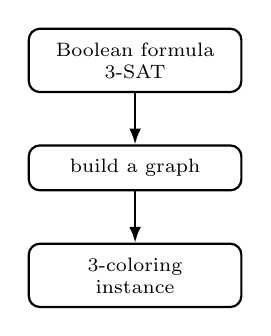
\begin{tikzpicture}[node distance=0.65cm]
    \node[box,minimum width=2.7cm] (sat) {Boolean formula\\3-SAT};
    \node[box,below=of sat,minimum width=2.7cm] (build) {build a graph};
    \node[box,below=of build,minimum width=2.7cm] (col) {3-coloring\\instance};
    \draw[arrow] (sat)--(build);
    \draw[arrow] (build)--(col);
\end{tikzpicture}
\vspace{0.2cm}
\small
The graph is colorable exactly when the formula is satisfiable.
\end{column}
\end{columns}
\end{frame}

% 3
\begin{frame}{P, NP, and NP-Complete}
\begin{columns}[T]
\begin{column}{0.53\textwidth}
\begin{itemize}
    \item \textbf{P}: problems solvable in polynomial time.
    \item \textbf{NP}: YES answers have certificates verifiable in polynomial time.
    \item \textbf{NP-hard}: at least as hard as every problem in NP.
    \item \textbf{NP-complete}: both in NP and NP-hard.
\end{itemize}
\vspace{0.25cm}
\textbf{Example certificates:}
\begin{itemize}
    \item 3-SAT: a truth assignment.
    \item 3-COLOR: a color for each vertex.
    \item CLIQUE: a set of selected vertices.
\end{itemize}
\end{column}
\begin{column}{0.43\textwidth}
\centering
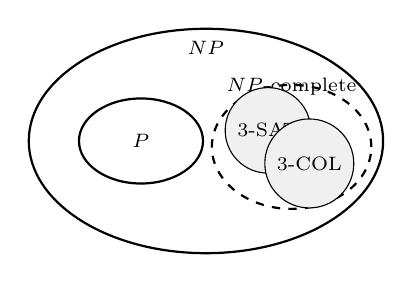
\begin{tikzpicture}[scale=0.75,every node/.style={font=\scriptsize}]
    \draw[thick] (0,0) ellipse (3.0 and 1.9);
    \node at (0,1.58) {$NP$};
    \draw[thick] (-1.1,0) ellipse (1.05 and 0.72);
    \node at (-1.1,0) {$P$};
    \draw[thick,dashed] (1.45,-0.10) ellipse (1.35 and 1.05);
    \node at (1.45,0.92) {$NP$-complete};
    \node[draw,circle,fill=black!6,minimum size=6mm] at (1.05,0.18) {3-SAT};
    \node[draw,circle,fill=black!6,minimum size=6mm] at (1.75,-0.38) {3-COL};
\end{tikzpicture}
\vspace{0.25cm}
\fbox{If one NP-complete problem is in P, then $P=NP$.}
\end{column}
\end{columns}
\end{frame}

% 4
\begin{frame}{Polynomial-Time Reduction}
\begin{columns}[T]
\begin{column}{0.54\textwidth}
A reduction
\[
A \le_p B
\]
means there is an efficient transformation $f$ such that
\[
x\in A \iff f(x)\in B.
\]
\vspace{0.15cm}
\textbf{Interpretation.} A solver for $B$ would also solve $A$ after the transformation.
\vspace{0.25cm}
\begin{block}{Direction matters}
To prove target problem $B$ is hard:
\[
\text{known NP-complete } A \le_p \text{ target } B.
\]
\end{block}
\end{column}
\begin{column}{0.42\textwidth}
\centering
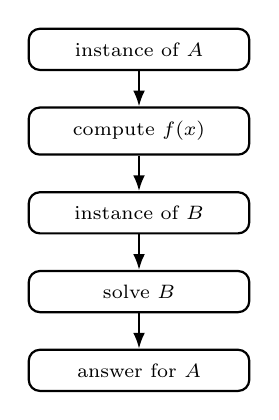
\begin{tikzpicture}[node distance=0.45cm]
    \node[box,minimum width=2.8cm] (a) {instance of $A$};
    \node[box,below=of a,minimum width=2.8cm] (f) {compute $f(x)$};
    \node[box,below=of f,minimum width=2.8cm] (b) {instance of $B$};
    \node[box,below=of b,minimum width=2.8cm] (s) {solve $B$};
    \node[box,below=of s,minimum width=2.8cm] (ans) {answer for $A$};
    \draw[arrow] (a)--(f);
    \draw[arrow] (f)--(b);
    \draw[arrow] (b)--(s);
    \draw[arrow] (s)--(ans);
\end{tikzpicture}
\end{column}
\end{columns}
\end{frame}

% 5
\begin{frame}{The Two Problems}
\begin{columns}[T]
\begin{column}{0.48\textwidth}
\begin{block}{3-SAT}
Given a Boolean formula in CNF with exactly 3 literals per clause:
\[
\phi=C_1\land C_2\land\cdots\land C_m.
\]
Question: is there a truth assignment satisfying all clauses?
\end{block}
\end{column}
\begin{column}{0.48\textwidth}
\begin{block}{3-COLORABILITY}
Given a graph $G$, can we color every vertex using only three colors so that adjacent vertices always have different colors?
\end{block}
\end{column}
\end{columns}
\vspace{0.25cm}
\begin{center}
\fbox{Theorem: $3\text{-SAT} \le_p 3\text{-COLORABILITY}$.}
\end{center}
\end{frame}

% 6
\begin{frame}{Reduction Plan: Build a Graph from a Formula}
\begin{center}
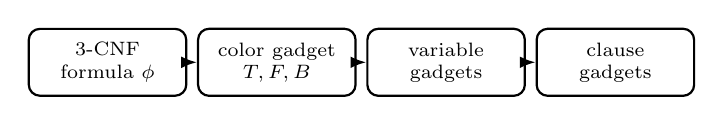
\begin{tikzpicture}[every node/.style={font=\scriptsize}]
    \node[box,minimum width=2.0cm] (phi) at (-3.2,0) {$3$-CNF\\formula $\phi$};
    \node[box,minimum width=2.0cm] (palette) at (-1.05,0) {color gadget\\$T,F,B$};
    \node[box,minimum width=2.0cm] (vars) at (1.10,0) {variable\\gadgets};
    \node[box,minimum width=2.0cm] (clauses) at (3.25,0) {clause\\gadgets};
    \draw[arrow] (phi)--(palette);
    \draw[arrow] (palette)--(vars);
    \draw[arrow] (vars)--(clauses);
\end{tikzpicture}
\end{center}
\vspace{0.25cm}
\begin{itemize}
    \item The color gadget gives fixed meanings to the three colors.
    \item Each variable gadget forces $x_i$ and $\neg x_i$ to take opposite truth values.
    \item Each clause gadget is colorable only when at least one of its literals is true.
\end{itemize}
\vspace{0.25cm}
\begin{center}
\fbox{$\phi$ is satisfiable $\iff$ constructed graph $G_\phi$ is 3-colorable.}
\end{center}
\end{frame}

% 7
\begin{frame}{Simulation Step 1: Color Gadget}
\begin{columns}[T]
\begin{column}{0.48\textwidth}
Create three special vertices $T,F,B$ and connect them as a triangle.
\vspace{0.2cm}
\begin{itemize}
    \item $T$ means the true color.
    \item $F$ means the false color.
    \item $B$ means base/helper color.
\end{itemize}
\vspace{0.2cm}
Because they form a triangle, all three must receive different colors.
\end{column}
\begin{column}{0.48\textwidth}
\centering
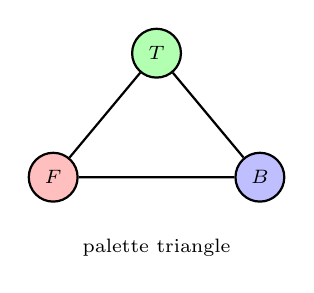
\begin{tikzpicture}[scale=1.05,every node/.style={font=\scriptsize}]
    \node[dot,fill=green!30] (T) at (0,1.5) {$T$};
    \node[dot,fill=red!25] (F) at (-1.25,0) {$F$};
    \node[dot,fill=blue!25] (B) at (1.25,0) {$B$};
    \draw[thick] (T)--(F)--(B)--(T);
    \node[align=center] at (0,-0.85) {palette triangle};
\end{tikzpicture}
\end{column}
\end{columns}
\end{frame}

% 8
\begin{frame}{Simulation Step 2: Variable Gadget}
\begin{columns}[T]
\begin{column}{0.46\textwidth}
For each variable $x_i$, create two vertices $x_i$ and $\neg x_i$.
\vspace{0.15cm}
\begin{itemize}
    \item Connect $x_i$ to $\neg x_i$.
    \item Connect both to the base vertex $B$.
\end{itemize}
\vspace{0.15cm}
Then $x_i$ and $\neg x_i$ cannot use the base color and cannot have the same truth color.
\end{column}
\begin{column}{0.50\textwidth}
\centering
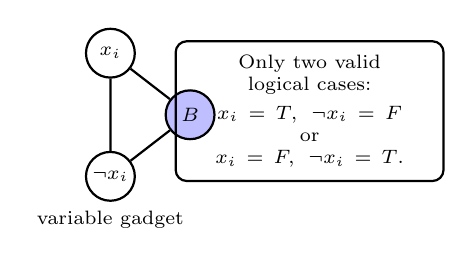
\begin{tikzpicture}[scale=0.92,every node/.style={font=\scriptsize}]
    \node[dot,fill=blue!25] (B) at (0,0) {$B$};
    \node[dot] (x) at (-1.1,0.85) {$x_i$};
    \node[dot] (nx) at (-1.1,-0.85) {$\neg x_i$};
    \draw[thick] (x)--(nx)--(B)--(x);
    \node[align=center] at (-1.1,-1.45) {variable gadget};
    \node[box,text width=3.05cm] at (1.65,0.05) {Only two valid logical cases:\\[0.08cm]
    $x_i=T,\; \neg x_i=F$\\or\\$x_i=F,\; \neg x_i=T$.};
\end{tikzpicture}
\end{column}
\end{columns}
\end{frame}

% 9
\begin{frame}{Simulation Step 3: Clause Gadget Interface}
\begin{columns}[T]
\begin{column}{0.46\textwidth}
For a clause
\[
(\ell_1\vee \ell_2\vee \ell_3),
\]
attach a constant-size OR gadget to the three literal vertices.
\vspace{0.15cm}
\begin{block}{Required property}
The gadget can be 3-colored exactly when at least one input literal has color $T$.
\end{block}
\end{column}
\begin{column}{0.50\textwidth}
\centering
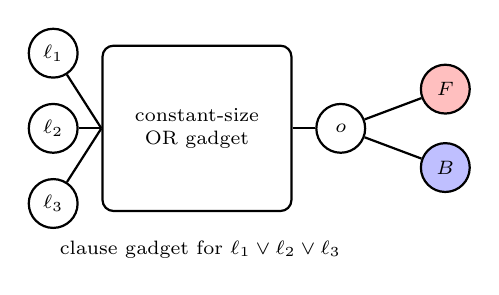
\begin{tikzpicture}[scale=0.83,every node/.style={font=\scriptsize}]
    \node[dot] (l1) at (0,2.0) {$\ell_1$};
    \node[dot] (l2) at (0,0.85) {$\ell_2$};
    \node[dot] (l3) at (0,-0.3) {$\ell_3$};
    \node[box,minimum width=2.4cm,minimum height=2.1cm] (or) at (2.2,0.85) {constant-size\\OR gadget};
    \node[dot] (out) at (4.4,0.85) {$o$};
    \node[dot,fill=red!25] (F) at (6.0,1.45) {$F$};
    \node[dot,fill=blue!25] (B) at (6.0,0.25) {$B$};
    \draw[thick] (l1)--(or.west);
    \draw[thick] (l2)--(or.west);
    \draw[thick] (l3)--(or.west);
    \draw[thick] (or.east)--(out);
    \draw[thick] (out)--(F);
    \draw[thick] (out)--(B);
    \node[align=center] at (2.25,-1.0) {clause gadget for $\ell_1\vee\ell_2\vee\ell_3$};
\end{tikzpicture}
\end{column}
\end{columns}
\end{frame}

% 10
\begin{frame}{Clause Gadget Truth Table}
\centering
\begin{tabular}{ccc|c|c}
\toprule
$\ell_1$ & $\ell_2$ & $\ell_3$ & clause value & gadget colorable? \\
\midrule
F & F & F & F & No \\
T & F & F & T & Yes \\
F & T & F & T & Yes \\
F & F & T & T & Yes \\
T & T & F & T & Yes \\
T & F & T & T & Yes \\
F & T & T & T & Yes \\
T & T & T & T & Yes \\
\bottomrule
\end{tabular}
\vspace{0.35cm}

\begin{center}
\fbox{The only forbidden case is when all three literals are false.}
\end{center}
\end{frame}

% 11
\begin{frame}{Simulation Formula}
Use the following small formula:
\[
\phi=(x_1\vee \neg x_2\vee x_3)\land(\neg x_1\vee x_2\vee \neg x_3).
\]
\vspace{0.15cm}
\begin{columns}[T]
\begin{column}{0.46\textwidth}
\begin{block}{Clauses}
\[
C_1=(x_1\vee \neg x_2\vee x_3)
\]
\[
C_2=(\neg x_1\vee x_2\vee \neg x_3)
\]
\end{block}
\end{column}
\begin{column}{0.46\textwidth}
\begin{block}{One satisfying assignment}
\[
x_1=T,
\quad x_2=T,
\quad x_3=F.
\]
Then $C_1$ is true by $x_1$, and $C_2$ is true by $x_2$ and $\neg x_3$.
\end{block}
\end{column}
\end{columns}
\end{frame}

% 12
\begin{frame}{Simulation Step 4: Assemble the Graph}
\centering
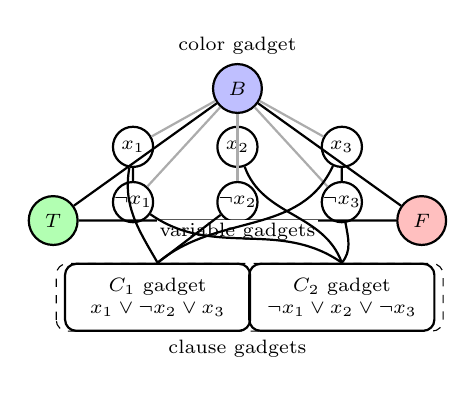
\begin{tikzpicture}[scale=0.78,every node/.style={font=\scriptsize}]
    % palette triangle
    \node[dot,fill=green!30] (T) at (-3.0,0.0) {$T$};
    \node[dot,fill=blue!25] (B) at (0,2.15) {$B$};
    \node[dot,fill=red!25] (F) at (3.0,0.0) {$F$};
    \draw[thick] (T)--(B)--(F)--(T);
    \node at (0,2.85) {color gadget};

    % variable gadgets
    \node[smalldot] (x1) at (-1.7,1.20) {$x_1$};
    \node[smalldot] (nx1) at (-1.7,0.30) {$\neg x_1$};
    \node[smalldot] (x2) at (0,1.20) {$x_2$};
    \node[smalldot] (nx2) at (0,0.30) {$\neg x_2$};
    \node[smalldot] (x3) at (1.7,1.20) {$x_3$};
    \node[smalldot] (nx3) at (1.7,0.30) {$\neg x_3$};

    \foreach \a/\b in {x1/nx1,x2/nx2,x3/nx3} {\draw[thick] (\a)--(\b);}
    \foreach \a in {x1,nx1,x2,nx2,x3,nx3} {\draw[gray!65,thick] (B)--(\a);}
    \node[fill=white,inner sep=1pt] at (0,-0.18) {variable gadgets};

    % clause gadget boxes
    \node[box,minimum width=2.35cm,minimum height=0.85cm] (c1) at (-1.3,-1.25) {$C_1$ gadget\\$x_1\vee\neg x_2\vee x_3$};
    \node[box,minimum width=2.35cm,minimum height=0.85cm] (c2) at (1.7,-1.25) {$C_2$ gadget\\$\neg x_1\vee x_2\vee\neg x_3$};
    \draw[dashed,rounded corners] (-2.95,-1.8) rectangle (3.35,-0.70);
    \node at (0,-2.08) {clause gadgets};

    % wires from literals to clauses
    \draw[thick] (x1) to[out=-100,in=120] (c1.north);
    \draw[thick] (nx2) -- (c1.north);
    \draw[thick] (x3) to[out=-115,in=40] (c1.north);
    \draw[thick] (nx1) to[out=-35,in=145] (c2.north);
    \draw[thick] (x2) to[out=-70,in=110] (c2.north);
    \draw[thick] (nx3) to[out=-80,in=50] (c2.north);
\end{tikzpicture}
\vspace{0.1cm}

\small Each clause gadget is connected only to the literal vertices appearing in that clause.
\end{frame}

% 13
\begin{frame}{Simulation Step 5: Assignment $\Rightarrow$ Coloring}
\begin{columns}[T]
\begin{column}{0.38\textwidth}
Take
\[
x_1=T,\quad x_2=T,\quad x_3=F.
\]
Color the literal nodes:
\[
x_1:T,\; \neg x_1:F
\]
\[
x_2:T,\; \neg x_2:F
\]
\[
x_3:F,\; \neg x_3:T
\]
Every clause has at least one true literal.
\end{column}
\begin{column}{0.58\textwidth}
\centering
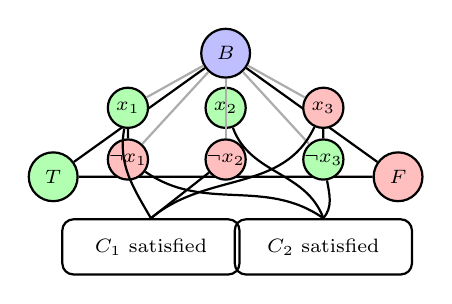
\begin{tikzpicture}[scale=0.73,every node/.style={font=\scriptsize}]
    \node[dot,fill=green!30] (T) at (-3.0,0.0) {$T$};
    \node[dot,fill=blue!25] (B) at (0,2.15) {$B$};
    \node[dot,fill=red!25] (F) at (3.0,0.0) {$F$};
    \draw[thick] (T)--(B)--(F)--(T);

    \node[smalldot,fill=green!30] (x1) at (-1.7,1.20) {$x_1$};
    \node[smalldot,fill=red!25] (nx1) at (-1.7,0.30) {$\neg x_1$};
    \node[smalldot,fill=green!30] (x2) at (0,1.20) {$x_2$};
    \node[smalldot,fill=red!25] (nx2) at (0,0.30) {$\neg x_2$};
    \node[smalldot,fill=red!25] (x3) at (1.7,1.20) {$x_3$};
    \node[smalldot,fill=green!30] (nx3) at (1.7,0.30) {$\neg x_3$};

    \foreach \a/\b in {x1/nx1,x2/nx2,x3/nx3} {\draw[thick] (\a)--(\b);}
    \foreach \a in {x1,nx1,x2,nx2,x3,nx3} {\draw[gray!65,thick] (B)--(\a);}

    \node[box,minimum width=2.25cm,minimum height=0.70cm] (c1) at (-1.3,-1.22) {$C_1$ satisfied};
    \node[box,minimum width=2.25cm,minimum height=0.70cm] (c2) at (1.7,-1.22) {$C_2$ satisfied};
    \draw[thick] (x1) to[out=-100,in=120] (c1.north);
    \draw[thick] (nx2) -- (c1.north);
    \draw[thick] (x3) to[out=-115,in=40] (c1.north);
    \draw[thick] (nx1) to[out=-35,in=145] (c2.north);
    \draw[thick] (x2) to[out=-70,in=110] (c2.north);
    \draw[thick] (nx3) to[out=-80,in=50] (c2.north);
\end{tikzpicture}
\end{column}
\end{columns}
\end{frame}

% 14
\begin{frame}{Correctness of the Reduction}
\begin{columns}[T]
\begin{column}{0.49\textwidth}
\begin{block}{$\phi$ satisfiable $\Rightarrow G_\phi$ 3-colorable}
\begin{itemize}
    \item Color $T,F,B$ in the palette triangle.
    \item For each variable, color the true literal with color $T$ and the false literal with color $F$.
    \item Since each clause has a true literal, every clause gadget can be extended to a legal coloring.
\end{itemize}
\end{block}
\end{column}
\begin{column}{0.49\textwidth}
\begin{block}{$G_\phi$ 3-colorable $\Rightarrow \phi$ satisfiable}
\begin{itemize}
    \item Each variable gadget forces exactly one of $x_i,\neg x_i$ to have color $T$.
    \item Set that literal to true.
    \item Each clause gadget being colorable implies at least one input literal is true.
\end{itemize}
\end{block}
\end{column}
\end{columns}
\vspace{0.2cm}
\begin{center}
\fbox{$\phi$ is satisfiable $\iff G_\phi$ is 3-colorable.}
\end{center}
\end{frame}

% 15
\begin{frame}{Quick Second Example: 3-SAT $\le_p$ CLIQUE}
\begin{columns}[T]
\begin{column}{0.46\textwidth}
\begin{itemize}
    \item Create one vertex for each literal occurrence.
    \item Put vertices in clause groups.
    \item Connect vertices from different clauses if they are not contradictory.
    \item Ask for a clique of size $m$.
\end{itemize}
\vspace{0.15cm}
\fbox{One compatible literal from each clause forms a clique.}
\end{column}
\begin{column}{0.50\textwidth}
\centering
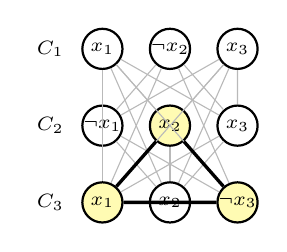
\begin{tikzpicture}[scale=0.78,every node/.style={font=\scriptsize}]
    \node[smalldot] (a) at (0,2.1) {$x_1$};
    \node[smalldot] (b) at (1.1,2.1) {$\neg x_2$};
    \node[smalldot] (c) at (2.2,2.1) {$x_3$};
    \node[smalldot] (d) at (0,0.85) {$\neg x_1$};
    \node[smalldot,fill=yellow!30] (e) at (1.1,0.85) {$x_2$};
    \node[smalldot] (f) at (2.2,0.85) {$x_3$};
    \node[smalldot,fill=yellow!30] (g) at (0,-0.4) {$x_1$};
    \node[smalldot] (h) at (1.1,-0.4) {$x_2$};
    \node[smalldot,fill=yellow!30] (i) at (2.2,-0.4) {$\neg x_3$};
    \draw[gray!55] (a)--(e); \draw[gray!55] (a)--(f); \draw[gray!55] (b)--(d); \draw[gray!55] (b)--(f);
    \draw[gray!55] (c)--(d); \draw[gray!55] (c)--(e); \draw[gray!55] (c)--(f);
    \draw[gray!55] (a)--(g); \draw[gray!55] (a)--(h); \draw[gray!55] (a)--(i); \draw[gray!55] (b)--(g); \draw[gray!55] (b)--(i); \draw[gray!55] (c)--(g); \draw[gray!55] (c)--(h);
    \draw[gray!55] (d)--(h); \draw[gray!55] (d)--(i); \draw[gray!55] (e)--(g); \draw[gray!55] (e)--(h); \draw[gray!55] (e)--(i); \draw[gray!55] (f)--(g); \draw[gray!55] (f)--(h);
    \draw[very thick] (e)--(g)--(i)--(e);
    \node[left=0.1cm of a] {$C_1$}; \node[left=0.1cm of d] {$C_2$}; \node[left=0.1cm of g] {$C_3$};
\end{tikzpicture}
\end{column}
\end{columns}
\end{frame}

% 16
\begin{frame}{Takeaway and References}
\begin{block}{Takeaway}
\begin{itemize}
    \item NP-completeness is proved using polynomial-time reductions.
    \item The reduction must preserve YES/NO answers.
    \item Gadget reductions encode logical constraints inside graph structure.
\end{itemize}
\end{block}
\begin{block}{References}
\begin{itemize}
    \item Michael Sipser, \emph{Introduction to the Theory of Computation}.
    \item Cormen, Leiserson, Rivest, Stein, \emph{Introduction to Algorithms}.
    \item CMU 15-451/651 lecture notes on NP-completeness.
    \item Stanford CS103 slides on 3-SAT to 3-COLOR gadgets.
\end{itemize}
\end{block}
\vspace{0.1cm}
\begin{center}
\small Thank you.
\end{center}
\end{frame}

\end{document}
